
\documentclass[10pt]{beamer}
\usepackage[utf8]{inputenc}
\usepackage[french]{babel}
\usepackage{multirow}
\usepackage{graphicx}
\usetheme{CambridgeUS}
\useoutertheme{infolines}
\usepackage{wasysym}

\title{Clean Architecture \& Python/Django}
\author{\textbf{Yann JACOB}}

\date{Décembre 2017}

\begin{document}

\maketitle

\frame{ 
    \frametitle{Principe}
    \begin{block}{Des problèmes rencontrés tous les jours...}
     \begin{itemize}
      \item Lire facilement les Use Cases, le domaine métier
      \item Avoir des tests réellement unitaires \tiny(AUCUN appel BDD, fichier, \ldots)\normalsize
      \item Dépendance aux choix techno initiaux
     \end{itemize}
    \end{block}
    \begin{alertblock}{Conséquences}
    \begin{itemize}
     \item Temps perdu pour comprendre le métier
     \item L'abandon des tests \tiny(ou peu de tests, ou des problème à l'intégration, \ldots)\normalsize
     \item Difficulté à faire évoluer le code
    \end{itemize}
    \end{alertblock}
}

\frame
{
    \frametitle{Principe}
    \begin{block}{Cas le plus courant}
    \begin{itemize}
     \item Imbrication entre logique métier, BDD, affichage, appels APIs externes, \ldots
     \item Lenteur \tiny(charger le framework, lancer une instance jetable BDD, \ldots)\normalsize
     \item Logique métier enfouie, difficile à reproduire dans un test
    \end{itemize}
    \end{block}
    \begin{alertblock}{Idée}
        \textbf{Le centre d'une application n'est pas le framework, ni la base de données, mais le domaine / les use case.}
    \end{alertblock}
}
\frame{ 
    \frametitle{Clean Architecture}
    \begin{block}{Origine}
    \begin{itemize}
     \item Robert C. Martin (Uncle Bob)
     \item Exemples en Java
    \end{itemize}
    \end{block}
    \begin{block}{Dans ce talk}
    \begin{itemize}
     \item Demo jouet Python / Django (gestion de paniers)
     \item \textbf{Pythonique - PEP20}
     \item Mon expérience sur des projets réels
    \end{itemize}
    \end{block}
}
\frame{ 
    \frametitle{Clean Architecture}
    \begin{block}{Comment}
    \begin{itemize}
     \item Logique métier = coeur application
     \item Logique métier isolée de la technique
     \item Détails techniques autour (BDD, Web, ressources externes, \ldots)
     \item Modèle en 4 couches
    \end{itemize}
    \end{block}
}
\frame{ 
    \frametitle{Clean Architecture}
    \begin{block}{Modèle en couches}
    \begin{figure}
    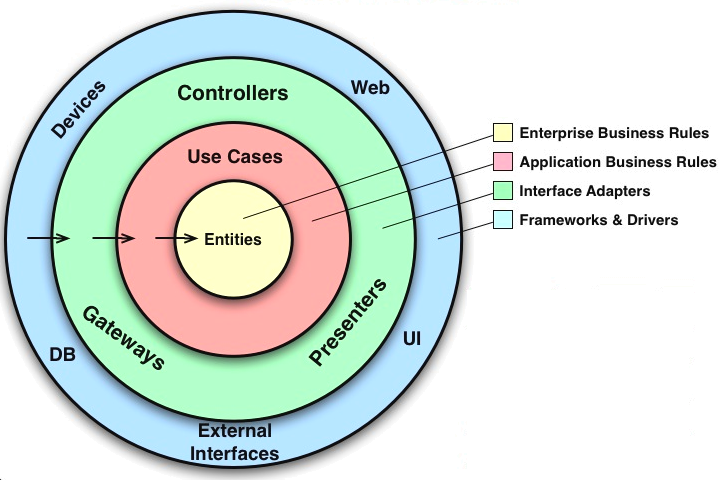
\includegraphics[width=8cm]{CleanArchitecture.png}
    \caption{Figure par Robert C. Martin}
    \end{figure}
    \end{block}
}
\frame{ 
    \frametitle{Couche 1: Entités}
    \begin{block}{Entités}
        \begin{itemize}
            \item Python pur, ni dépendances ni objets externes
            \item Classe entités du domaine métier
            \item Fournit explicement toutes les règles métier
            \item Exception = violation de règle
            \item Compatible DDD, TDD
        \end{itemize}
    \end{block}
}
\frame{ 
    \frametitle{Couche 1: Entités (modules/entities/product)}
    \begin{block}{Entités: Produit}
        \begin{itemize}
            \item Le nom doit être des lettres puis des chiffres
            \item Prix strictement positif
            \item Nombre de produits réservés (dans les paniers) et disponibles
            \item Conversion monétaire
        \end{itemize}
    \end{block}
}
\frame{ 
    \frametitle{Couche 1: Entités (modules/entities/cart)}
    \begin{block}{Entités: Panier}
        \begin{itemize}
            \item Liste de produits achetés avec le nombre (positif!)
            \item Conversion monétaire / valeur totale
            \item Exercice: 25 euros de montant minimum de panier
        \end{itemize}
    \end{block}
}
\frame{ 
    \frametitle{Couche 2: Cas d'Usage}
    \begin{block}{Cas d'Usage}
        \begin{itemize}
            \item Python pur, ni dépendances ni objets externes
            \item Fonctions cas d'usage métiers explicites
            \item Cas d'usage trivaux shuntés dans la démo (getters/setters/etc.)
        \end{itemize}
    \end{block}
}
\frame{ 
    \frametitle{Couche 2: Cas d'Usage (modules/usecases/fill\_cart)}
    \begin{block}{Cas d'Usage: remplir panier}
        Trois choses à faire:
        \begin{itemize}
            \item 1) Retirer le nombre de la liste des produits disponibles
            \item 2) Ajout le nombre à la la listes produits réservés
            \item 3) Ajouter dans le panier
        \end{itemize}
    \end{block}
}
\frame{ 
    \frametitle{Couche 2: Cas d'Usage (modules/usecases/fill\_available\_products)}
    \begin{block}{Cas d'Usage: autres}
        \begin{itemize}
         \item Ajouter des produits disponibles
         \item Exercice: détruire un panier (penser à rendre au stock)
        \end{itemize}
    \end{block}
}
\frame{ 
    \frametitle{Couche 3: Adapteurs}
    \begin{block}{Présentation}
        \begin{itemize}
            \item Le liant entre les couches métier, et les briques techniques
            \item Présentation: fournit les différentes vues des entités
            \item Répertoires: sélectionne la source de données selon l'objets
            \item Controlleurs divers et variés
        \end{itemize}
    \end{block}
}
\frame{ 
    \frametitle{Couche 3: Présentation (modules/presentation)}
    \begin{block}{Présentation}
        \begin{itemize}
            \item Différentes présentations pour une donnée (JSON, XML, \ldots)
            \item Choisir quel champs afficher (nb\_available et nb\_reserved sont cachés)
        \end{itemize}
    \end{block}
}
\frame{ 
    \frametitle{Couche 4: Couches Techniques}
    \begin{block}{Couches Techniques}
    \begin{itemize}
     \item Les interfaces externes à l'application
     \item Notamment Django intervient ici
     \item Base de données, interface Web, API HTTP, \ldots
     \item Note: Django peut servir sans avoir besoin de BDD
    \end{itemize}
    \end{block}
}
\frame{ 
    \frametitle{Couche 4: Base de données (postgres\_api)}
    \begin{block}{Base de données (postgres\_api)}
    \begin{itemize}
     \item postgres\_api/models: le modèle
     \item postgres\_api/queries: requêtes pour interagir avec la BDD
     \item Les appels retournent toujours des entités
     \item Jamais d'objet BDD hors de ce répertoire
     \item Testé avec UnitTest de Django
    \end{itemize}
    \end{block}
}
\frame{ 
    \frametitle{Couche 4: Appel API externe (http\_api)}
    \begin{block}{Couche 4: Appel API externe (http\_api)}
     \begin{itemize}
      \item Appel à une API REST externe pour le taux de conversion euro-dollar en temps réel
      \item Mettre euro-dollar-rate.json dans localhost pour simuler un appel HTTP externe
      \item Définit la stratégie d'appels HTTP, de gestion des erreurs
      \item Outillage de test à définir, adapté au cas
     \end{itemize}
    \end{block}
}
\frame{ 
    \frametitle{Couche 4: Vue Web}
    \begin{block}{Couche 4: Vue Web}
    \begin{itemize}
     \item /Web pour la config
     \item /Webapps pour les applis
     \item /Webapps/API: example Django Rest Framework / Swagger
     \item Un site web pourrait se greffer facilement en plus de l'API
    \end{itemize}
    \end{block}
}
\frame{
    \frametitle{Couche 4: Vue Web (webapps/API/views)}
    \begin{block}{Couche 4: Vue Web(webapps/API/views)}
    \begin{itemize}
     \item wrapper exception métier - messages d'erreurs
     \item Le comportement REST attendu est défini ici
     \item Les méthodes font le liant entre entités, use cases, présentation, BDD, API
    \end{itemize}
    \end{block}
}
\frame{ 
    \frametitle{Conclusion}
    \begin{block}{Les forces}
     \begin{itemize}
      \item Domaine et règles métiers évidents
      \item Tester sans prise de tête (quasiment tout en pre-commit!)
      \item La stack Django fonctionne bien
      \item Migration MongoDB $\rightarrow$ PostGres triviale
      \item Stratégies d'appel HTTP, de présentation REST, de la gestion d'erreurs, d'optimsation des appels BDD, \ldots groupées à 1 endroit
     \end{itemize}
    \end{block}
}
\frame{ 
    \frametitle{Conclusion}
     \begin{block}{Les limitations}
     \begin{itemize}
      \item Surtout utile pour les projets moyens/gros avec de la logique métier
      \item Objets passe plat, beaucoup d'objets (shuntez les coquilles vides!)
      \item Quelques hacks sur Django (faux projet postgres\_api, structuration inhabituelle)
      \item Incompactible avec d'autres frameworks
     \end{itemize}
    \end{block}
}
\frame{ 
    \frametitle{Conclusion}
    \begin{block}{Perspectives}
    \begin{itemize}
     \item Extension de Django créeant le bon squelette from scratch ?
     \item Explorer de façon plus complète les concepts théoriques et adapter à python
    \end{itemize}
    \end{block}
}
\end{document}
